\subsection{Results}\label{subsec:results}
The models are evaluated using 3 different methods.

For training purposes the models are autoencoding a pose and the MSE between the original pose and the autoencoded pose gives a loss for training. This is a good baseline for training, but the actual interest lies around interpolation between poses.

Taking a motion and autoencoding each pose gives a good visual indication of how well the model manages coherency between related poses. This is important for animation as large gaps between poses around the same time interval gives a very jittery motion.

Performing in-painting on a motion, gives a visual indication as well as a numerical indication of how well the model performs. The in-painting is done by iterating through a motion and replacing the data between two poses with a linear interpolation of the two poses or an interpolation in latent space using a model. In-painting is done with increasing intervals of gaps in the motion. For small gaps, such as 1-4 frames, linear interpolation is likely going to perform near perfect, but for larger gaps, such as 32 frames, knowledge of human walking is required to fill the gap correctly.

\subsubsection{Autoencoder}\label{subsubsec:ae}
Two models are trained. One model has a small latent space (8 dimensions), while the other has a large latent space (128 dimensions).

The model with a large latent space becomes very good at autoencoding poses, as can be seen by the loss in \autoref{fig:ae-loss-large}. This is also evident in the very smooth autoencoded motion seen in \autoref{fig:ae-large-motion}. \autoref{fig-large-inpainting} shows a visualization of the motion inpainting, which reveals a problem with the large latent space. The model seems to encode rotations in a way that is so similar to the original rotations that the interpolation in latent space is almost identical to the interpolation in the motion space. This can also be seen in the comparison in \autoref{tab:ae-eval-large}.

In an effort to combat this issue a model was trained with a smaller latent space. This model did not achieve as high of an accuracy as the model with the large latent space, but it is sufficient for comparison. Furthermore there is a large gap in accuracy on training vs test data. This can be explained by poses in the test dataset being very far away from the train dataset, \autoref{fig:test-turning} shows an example of such a motion in the test dataset. Having a larger dataset would help alleviate this. \autoref{tab:ae-eval-small} shows a slightly worse performance on in-painting, but this likely a result of the model not being as good at autoencoding poses. \autoref{fig:ae-small-inpainting} and \autoref{fig:ae-small-motion} shows that while the model autoencodes the poses pretty well it lacks the ability to blend smoothly between similar poses, resulting in very jittery motion. This motivates the training of a VAE.





\begin{figure}[h]
    \centering
    \begin{subfigure}[t]{0.5\textwidth}
        \centering
        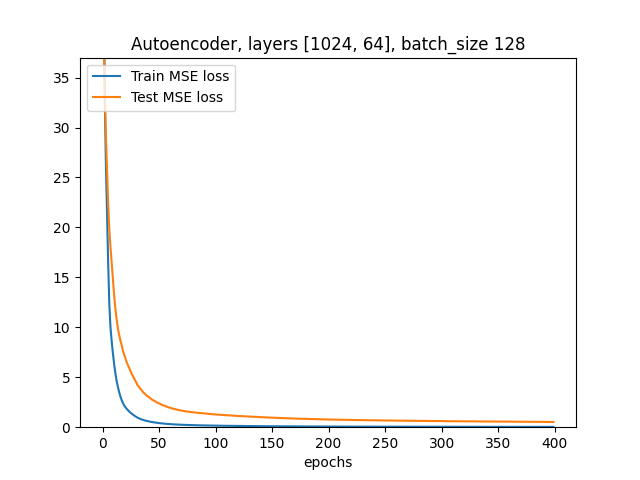
\includegraphics[height=5cm]{img/simple_1024-64_batch-128_losses}
        \caption{Loss over epochs for the model with a large latent space.}
    \label{fig:ae-loss-large}
    \end{subfigure}%
    ~
    \begin{subfigure}[t]{0.5\textwidth}
        \centering
        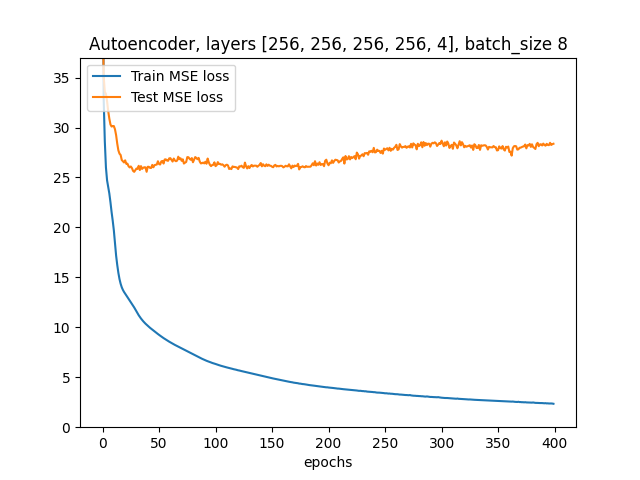
\includegraphics[height=5cm]{img/simple_256-256-256-256-4_batch-8_losses}
        \caption{Loss over epochs for the model with a small latent space.}
    \label{fig:ae-loss-small}
    \end{subfigure}
    \caption{MSE loss of autoencoding a pose for training and test datasets for the two autoencoder models.}
\end{figure}


\begin{figure}[h]
\centering
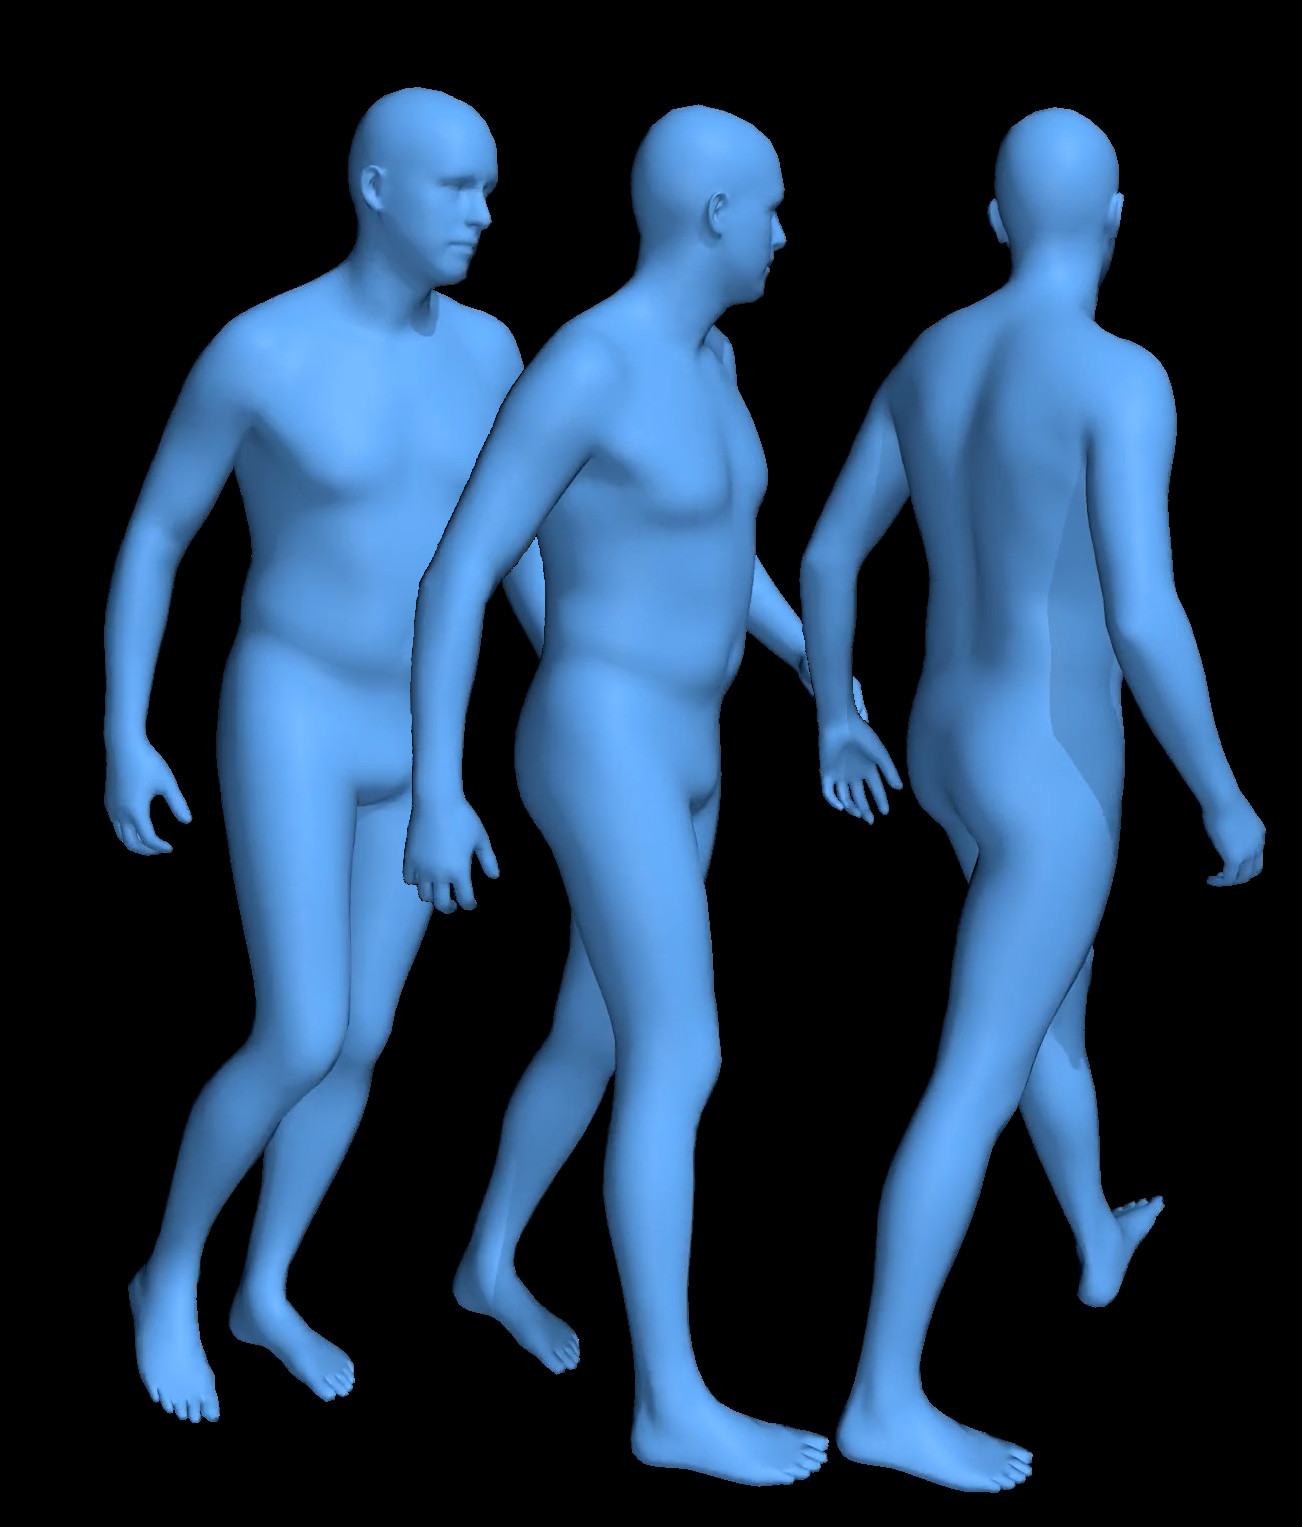
\includegraphics[width=0.3\textwidth]{img/46_01_turning}
\caption{Subject 46, trial 1 from the CMU dataset. The motion depicts turning around, as opposed to simply walking straight ahead.}
\label{fig:test-turning}
\end{figure}


\begin{table}[h]
    \begin{subtable}[h]{0.45\textwidth}
        \centering
        \begin{tabular}{@{}llll@{}}
        \toprule
        Step & Latent loss & Linear loss & Difference \\ \midrule
1 & 0.000000 & 0.000000 & 0.000000 \\
2 & 0.000004 & 0.000002 & -0.000002 \\
4 & 0.000008 & 0.000006 & -0.000002 \\
8 & 0.000029 & 0.000027 & -0.000002 \\
16 & 0.000142 & 0.000136 & -0.000006 \\
32 & 0.001255 & 0.001255 & 0.000000 \\
64 & 0.003744 & 0.003736 & -0.000008 \\
128 & 0.011174 & 0.011202 & 0.000028 \\ \bottomrule
        \end{tabular}
        \caption{Comparison for the model with a large latent space.}
        \label{tab:ae-eval-large}
    \end{subtable}
    \hfill
    \begin{subtable}[h]{0.45\textwidth}
        \centering
        \begin{tabular}{@{}llll@{}}
        \toprule
        Step & Latent loss & Linear loss & Difference \\ \midrule
1 & 0.000000 & 0.000000 & 0.000000 \\
2 & 0.000169 & 0.000002 & -0.000168 \\
4 & 0.000307 & 0.000006 & -0.000301 \\
8 & 0.000497 & 0.000027 & -0.000470 \\
16 & 0.000825 & 0.000136 & -0.000689 \\
32 & 0.002039 & 0.001255 & -0.000784 \\
64 & 0.005852 & 0.003736 & -0.002117 \\
128 & 0.011285 & 0.011202 & -0.000083 \\  \bottomrule
        \end{tabular}
        \caption{Comparison for the model with a small latent space.}
        \label{tab:ae-eval-small}
    \end{subtable}
     \caption{Comparison of loss using an interpolation in latent space and an interpolation in the motion space on a single motion from the test dataset. Step denotes the distance between the start pose and end pose in frames. TODO: FILL IN VALUES}
     \label{tab:ae-eval}
\end{table}




\subsubsection{Variational autoencoder}\label{subsubsec:vae}
A VAE is trained using a small latent space in order to avoid the issues around large latent spaces described in \autoref{subsubsec:ae}. It achieves a similar accuracy and has the same gap between test and train loss as the autoencoder with a small latent space, as can be seen in \autoref{fig:vae-loss}.

Comparing \autoref{fig:vae-motion} and \autoref{fig:ae-small-motion} it becomes clear that the variational encoder is capable of blending between latents space without jitter, showing the difference between a regular autoencoder and a VAE.

\autoref{fig:vae-inpainting} shows the result of in-painting a motion using this model. As can be seen, motion of the legs that have been interpolated using this model is actually closer to the real motion than to that of the linear interpolation. This suggests that the model is not just blindly trying to compress rotations, but that it has actually learned something about what a human walking motion looks like. What is also evident is the fact that the motion has various artifacts, such as spurious arm movement. This is probably because the model struggles to autoencode poses accurately and also the likely reason why the model does not score higher than the linear interpolation in \autoref{tab:vae-eval}. This suggests that a higher accuracy variation autoencoder would likely be able to perform motion in-painting/interpolation for human walking motion.

\begin{figure}[h]
\centering
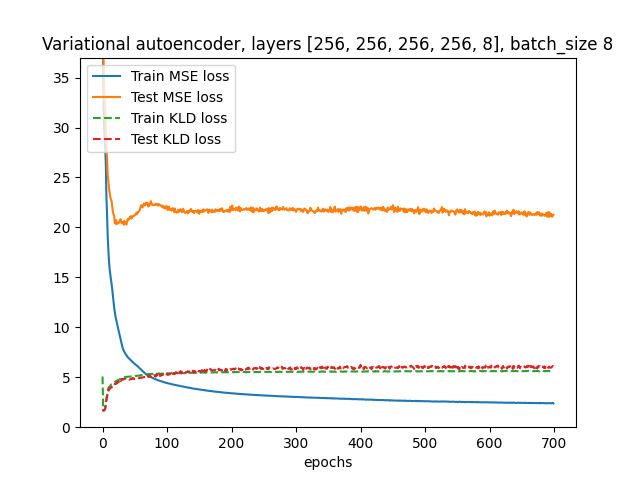
\includegraphics[width=0.5\textwidth]{img/vae_256-256-256-256-8_batch-8_losses}
\caption{MSE loss of autoencoding a pose and KLD loss for both the training and test datasets.}
\label{fig:vae-loss}
\end{figure}

\begin{table}[h]
\centering
\begin{tabular}{@{}llll@{}}
\toprule
Step & Latent loss & Linear loss & Difference  \\ \midrule
1    & 0.000000    & 0.000000    & 0.000000    \\
2    & 0.021803    & 0.000002    & -0.021801   \\
4    & 0.032558    & 0.000006    & -0.032552   \\
8    & 0.037987    & 0.000027    & -0.037960   \\
16   & 0.039968    & 0.000136    & -0.039831   \\
32   & 0.041304    & 0.001255    & -0.040048   \\
64   & 0.038672    & 0.003736    & -0.034937   \\
128  & 0.038981    & 0.011202    & -0.027780   \\ \bottomrule
\end{tabular}
\caption{Comparison of loss using an interpolation in latent space and an interpolation in the motion space on a single motion from the test dataset. Step denotes the distance between the start pose and end pose in frames.}
\label{tab:vae-eval}
\end{table}




\subsection{Further research}\label{subsec:further-research}
clustered-specialists-paper~\cite{won2020scalable}

something about motion prediction maybe (a way to utilize forwards/backwards info)

closer comparison with existing motion prediction models

using vq-vae

using the full amass data training
